% References
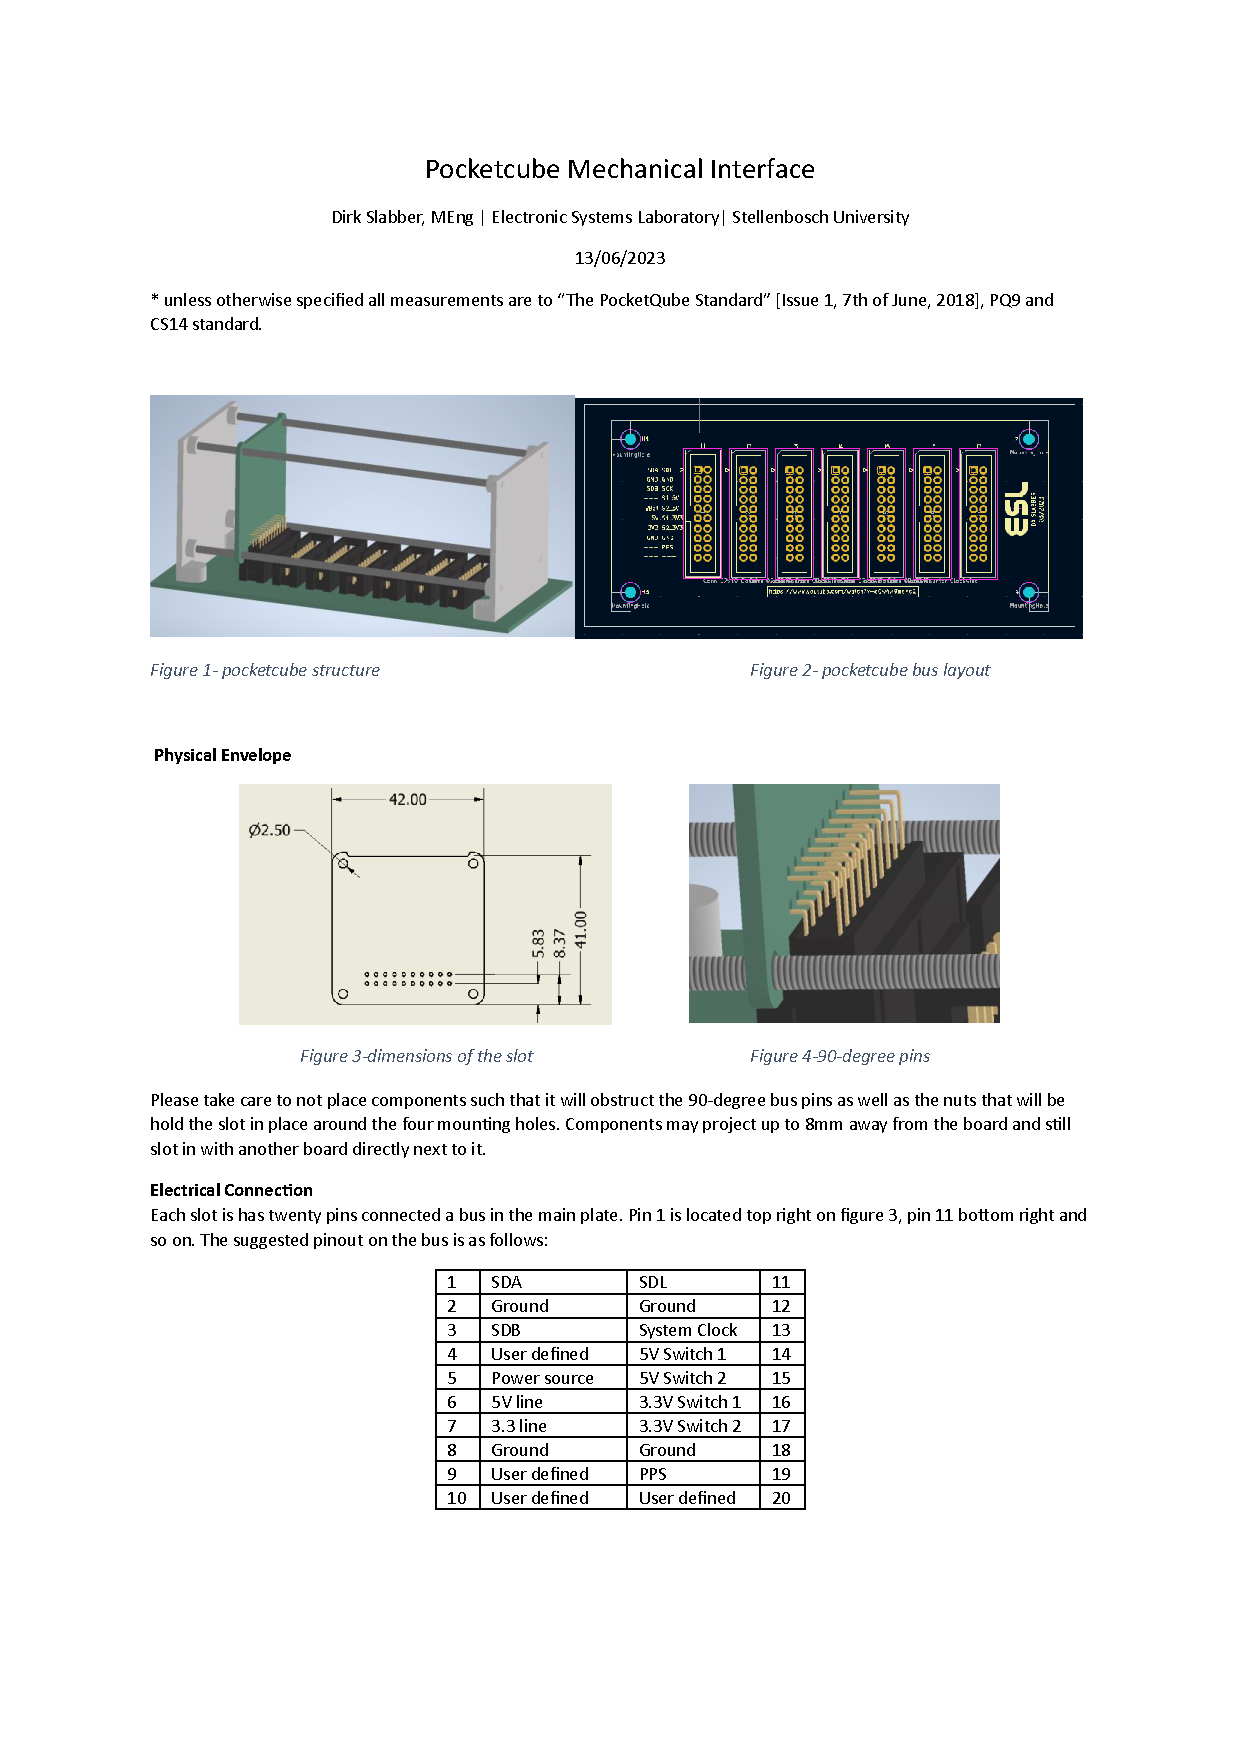
\includepdf[scale=0.8,pages=1,offset=0mm -35mm,pagecommand=\chapter{References}\section{PQSU}\label{sec:appendix_pqsu}]{docs/pqsu}
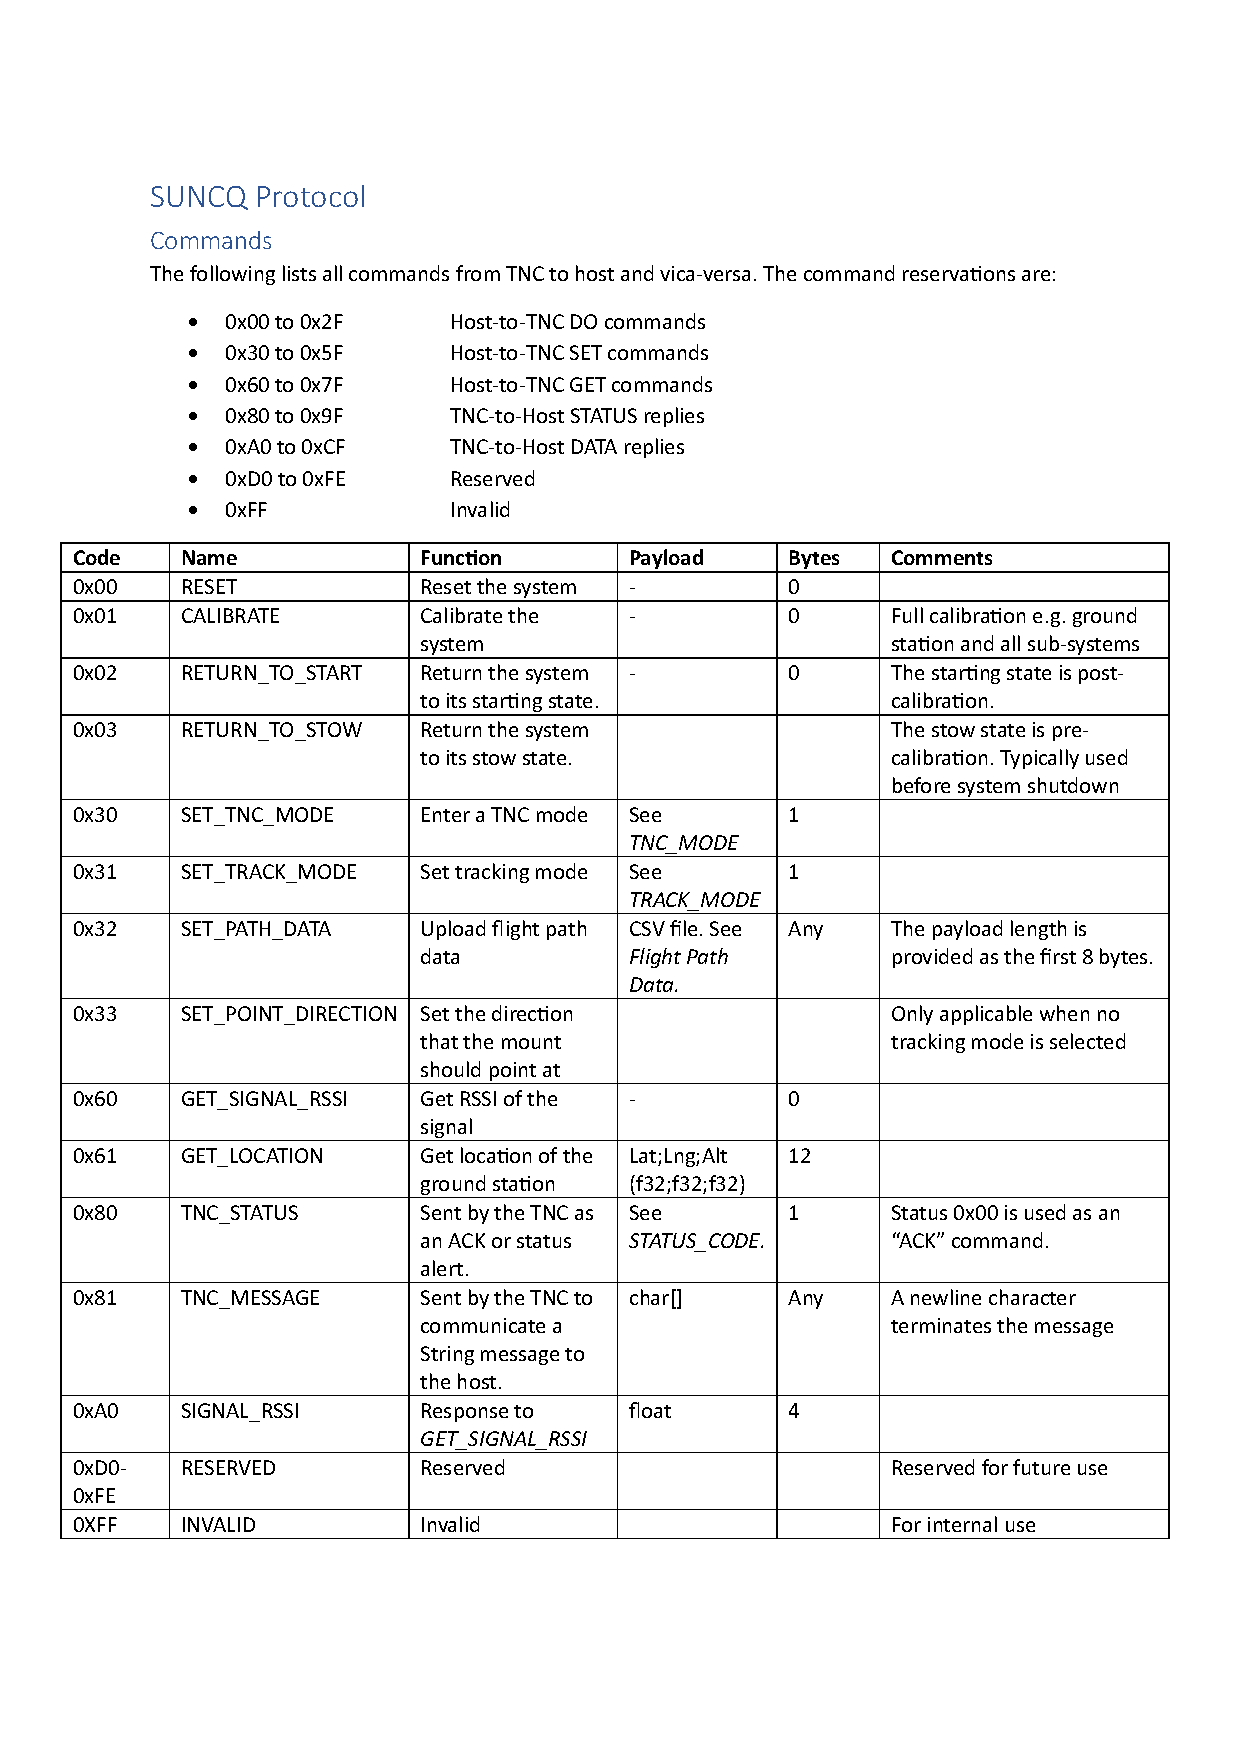
\includepdf[scale=0.85,pages=1,pagecommand=\section{SUNCQ}\label{sec:appendix_suncq}]{docs/suncq}
\includepdf[scale=0.85,pages=2]{docs/suncq}

\section{Antenna Comparison}
\begin{table}[!htb]
  \centering
  \renewcommand{\arraystretch}{1.2}
  \hspace*{-0.8cm}
  \begin{tabular}{ |c|c|c|c|c|c|c| }
  \hline
  \textbf{Type} & \textbf{Gain (dBi)} & \textbf{Beamwidth} & \textbf{Bandwidth} & \textbf{Size} & \textbf{Polarization} \\ \hline
  $0.5 \lambda$ Dipole & 2.15 & Omni-directional & Medium & Medium & Linear \\ \hline
  Monopole & 5.15 & Omni-directional & Small & Small & Linear \\ \hline
  Helical & $<20$ & Either & Large (50 - 60\%) & Small-Medium & Circular \\ \hline
  Microstrip & $<10$ & Either & Small-Medium & Small & Either \\ \hline
  Yagi-Uda & $<40$ & Uni-directional & Small & Large & Linear \\ \hline
  \end{tabular}
  \caption{Qualitative Comparison of Antenna Characteristics \cite{site-antennaTheory}}
  \label{tab:antenna_characteristics}
\end{table}

\section{Link Configuration Summary}
\begin{table}[!htb]
    \centering
    \renewcommand{\arraystretch}{1.2}
    \begin{tabular}{ |c|c|c|c|c| }
    \hline
    \textbf{Description} & \textbf{Modulation} & \textbf{Parameters} & \textbf{Bit Rate} & \textbf{Sensitivity} \\
    \hline
    Maximum Bit Rate &
    GFSK &
    62.5 kHz &
    250 000 bps &
    -92 dBm \\
    \hline
    High Bit Rate &
    GFSK &
    40 kHz &
    38400 bps &
    -109 dBm \\
    \hline
    Target Bit Rate ($\approx 9600 bps$) &
    GFSK &
    5 kHz &
    4800 bps &
    -115 dBm \\
    \hline
    - &
    LoRa &
    500 kHz, SF 8 &
    10417 bps &
    -119 dBm \\
    \hline
    Maximum Sensitivity &
    LoRa &
    62.5 kHz, SF 12 &
    24 bps &
    -147 dBm \\
    \hline
    \end{tabular}
    \caption{Notable SX1278 Configurations \cite{datasheet-SX1278}}
    \label{tab:sensitivity_values}
  \end{table}